\documentclass{article}

\renewcommand{\familydefault}{\sfdefault}  %serifenlose Schrift
\usepackage{helvet} % Schrift: Helvetica


\usepackage{graphicx,graphics,tikz}
\usepackage{amsmath}
\usepackage{amsthm}
\usepackage{amsfonts}
\usepackage{amssymb}
\usepackage{marvosym} % to be able to show male and female symbols with: \Female and \Male
\usepackage{gensymb}
\usepackage[graphics,tightpage,active]{preview}
\definecolor{spain}{rgb}{0.2,0.87,0.93}
\definecolor{france}{rgb}{0.4,0.2,0.6}
\definecolor{denmark}{rgb}{1,0.87,0.07}
\definecolor{norway}{rgb}{0.2,0.4,0}

\PreviewEnvironment{tikzpicture}
\newlength\imagewidth
\newlength\imagescale

\begin{document}

%\pgfmathsetlength{\imagewidth}{10cm} % desired displayed width of image
%\pgfmathsetlength{\imagescale}{\imagewidth/2000} % pixel width of image
% adjust scale of tikzpicture (and direction of y) such that pixel
% coordinates can be used for drawing overlays:
\usetikzlibrary{backgrounds}

\begin{tikzpicture}[scale=0.5]
\scalebox{0.52}{
\begin{scope}[xshift=-4cm]
\draw [-latex,line width=0.03cm](-10cm,0cm) --(10cm,0cm);

\draw [line width=0.03cm](-10cm,0cm) -- (-10cm,-0.5cm) node [anchor=north,scale=1.3] {0};
\draw [line width=0.03cm](-8cm,0cm) -- (-8cm,-0.5cm) node [anchor=north,scale=1.3] {4};
\draw [line width=0.03cm](-6cm,0cm) -- (-6cm,-0.5cm) node [anchor=north,scale=1.3] {8};
\draw [line width=0.03cm](-4cm,0cm) -- (-4cm,-0.5cm) node [anchor=north,scale=1.3] {12};
\draw [line width=0.03cm](-2cm,0cm) -- (-2cm,-0.5cm) node [anchor=north,scale=1.3] {16};
\draw [line width=0.03cm](0cm,0cm) -- (0cm,-0.5cm) node [anchor=north,scale=1.3] {20};
\draw [line width=0.03cm](2cm,0cm) -- (2cm,-0.5cm) node [anchor=north,scale=1.3] {24};
\draw [line width=0.03cm](4cm,0cm) -- (4cm,-0.5cm) node [anchor=north,scale=1.3] {28};
\draw [line width=0.03cm](6cm,0cm) -- (6cm,-0.5cm) node [anchor=north,scale=1.3] {32};
\draw [line width=0.03cm](8cm,0cm) -- (8cm,-0.5cm) node [anchor=north,scale=1.3] {36};
\node [anchor=north] at (11cm,0cm) [scale=1.3] {\celsius};

\node  [anchor=west,color=norway,scale=1.5] at (2cm,4.1cm) {\scriptsize{Norway}};
\node  [anchor=west,color=denmark,scale=1.5] at (2cm,3.1cm) {\scriptsize{Denmark}};
\node  [anchor=west,color=france,scale=1.5] at (2cm,2.1cm) {\scriptsize{Brittany}};
\node  [anchor=west,color=spain,scale=1.5] at (2cm,1.1cm) {\scriptsize{Spain}};

\draw [color=norway,line width=0.05cm](-10cm+0.5*-1.102cm,4cm) --(-10cm+0.5*11.927cm,4cm) node [anchor=south,color=norway]{};
\draw [color=denmark,line width=0.05cm](-10cm+0.5*6.336cm,3cm) --(-10cm+0.5*18.551cm,3cm) node [anchor=south,color=denmark]{};
\draw [color=france,line width=0.05cm](-10cm+0.5*13.425cm,2cm) --(-10cm+0.5*23.915cm,2cm) node [anchor=south,color=france]{};
\draw [color=spain,line width=0.05cm](-10cm+0.5*16.229cm,1cm) --(-10cm+0.5*23.138cm,1cm) node [anchor=south,color=spain]{};

\draw [color=norway,fill=norway] (-10cm+4.767*0.5cm,4cm) circle (0.15cm);
\draw [color=denmark,fill=denmark] (-10cm+11.882*0.5cm,3cm) circle (0.15cm);
\draw [color=france,fill=france] (-10cm+17.741*0.5cm,2cm) circle (0.15cm);
\draw [color=spain,fill=spain] (-10cm+18.688*0.5cm,1cm) circle (0.15cm);

\node [scale=1.5,anchor=west] at (-14cm,5.8cm){Thermal range in year 2200};

\node [scale=1.5,anchor=west] at (-14cm,-3cm){Measured response};


\end{scope}
}

\node[anchor=north west,inner sep=0pt,outer sep=0pt,scale=1] at (-12,-2.5) {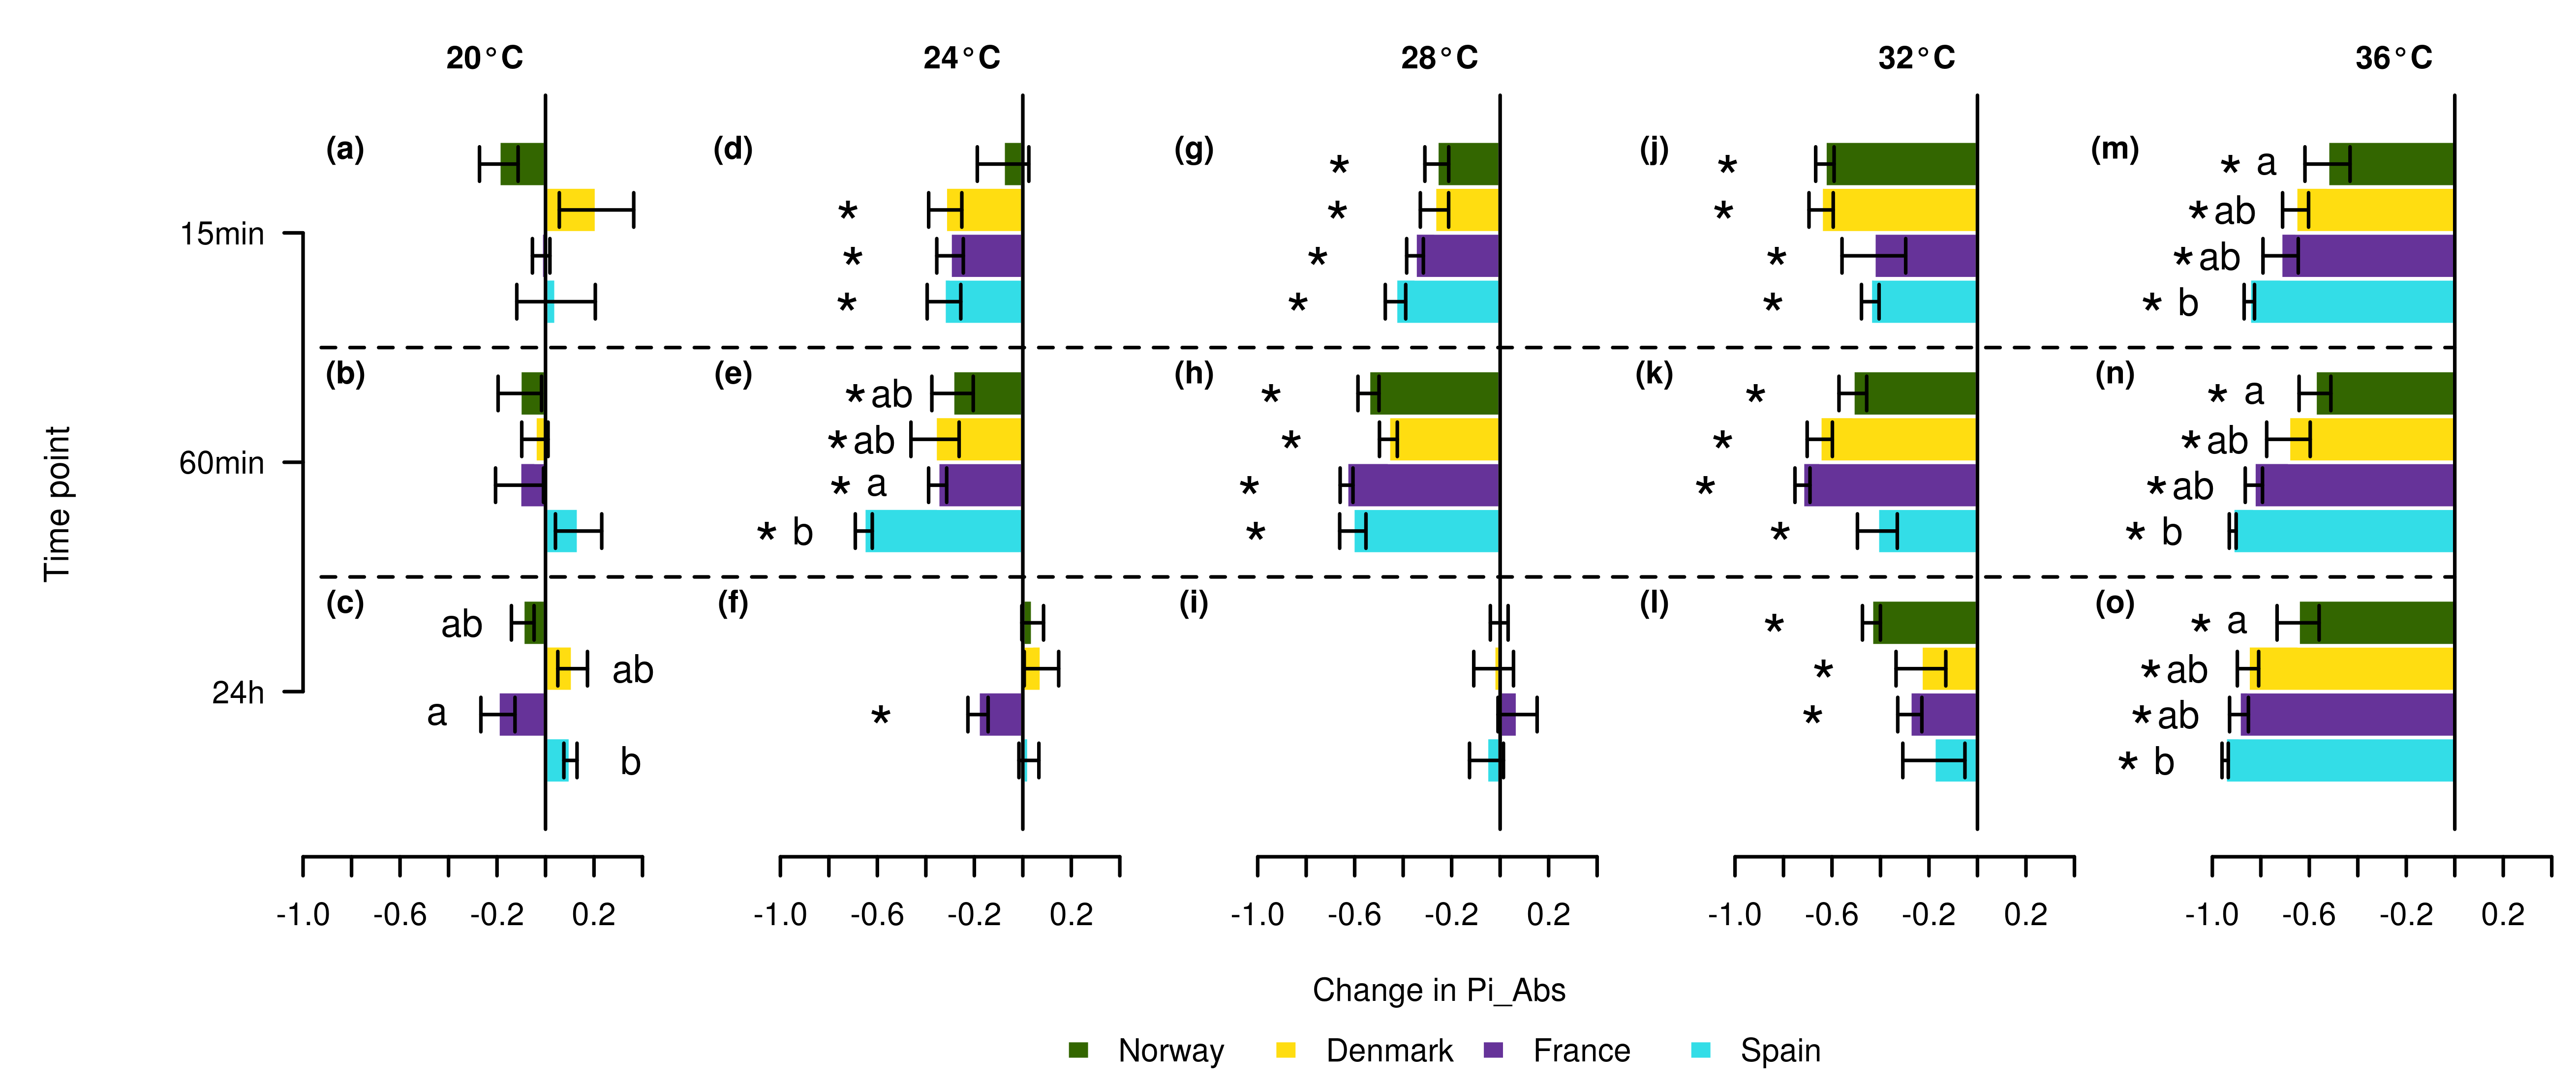
\includegraphics[width=11.5cm]{Fig2_color.png}};

\draw [dashed,line width=0.01cm] (-7,-2.8)--(-2.6,-1.1);
\draw [dashed,line width=0.01cm] (-7+4.1,-2.8)--(-2.6+1.3,-1.1);
\draw [dashed,line width=0.01cm] (-7+2*4.1,-2.8)--(-2.6+2*1.3,-1.1);
\draw [dashed,line width=0.01cm] (-7+3*4.1,-2.8)--(-2.6+3*1.3,-1.1);
\draw [dashed,line width=0.01cm] (-7+4*4.1,-2.8)--(-2.6+4*1.3,-1.1);



\begin{scope}[yshift=-1.3cm]
\begin{scope}[xshift=0cm,yshift=4cm]

\node[anchor=north west,inner sep=0pt,outer sep=0pt,scale=1] at (3.5,0) {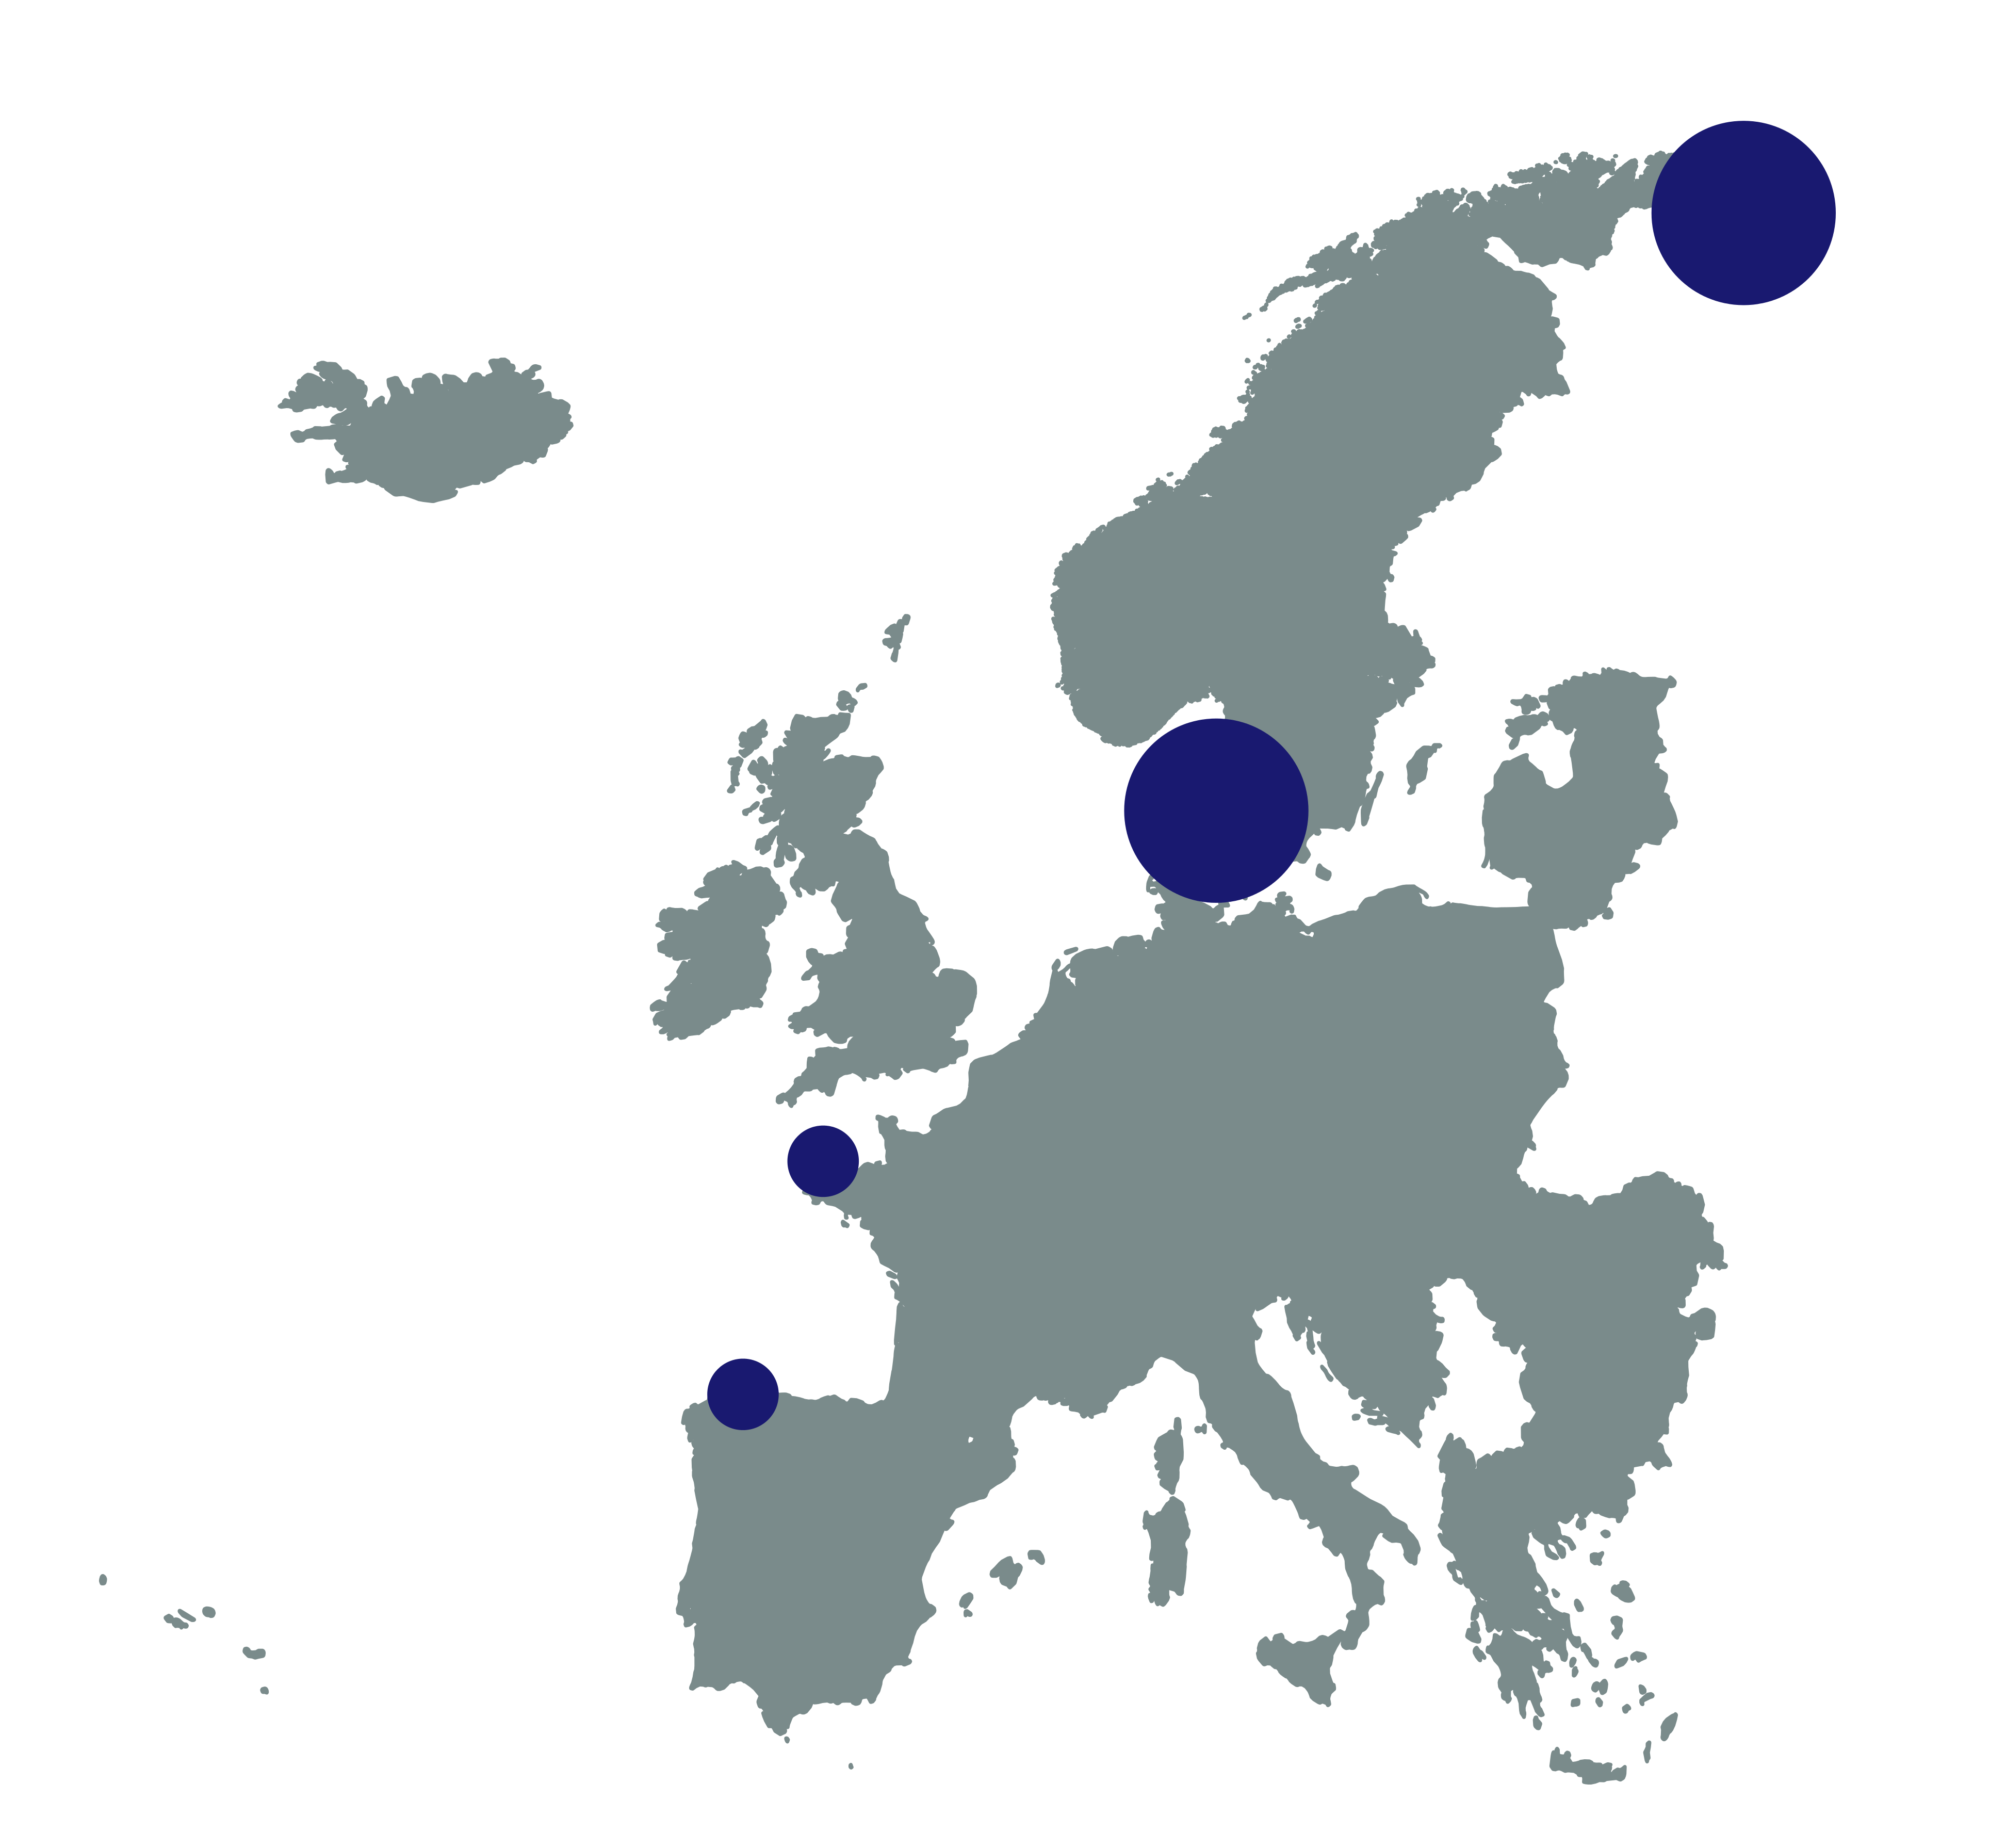
\includegraphics[width=2cm]{Performance.png}};
\begin{scope}[xshift=2.5cm, yshift=0.5cm]
\draw [color=norway,fill=norway] (4.49,-0.93cm) circle (0.2cm);
\draw [color=denmark,fill=denmark] (3.48,-2.1cm) circle (0.2cm);
\draw [color=france,fill=france] (2.65,-2.8cm) circle (0.08cm);
\draw [color=spain,fill=spain] (2.49,-3.3cm) circle (0.08cm);
\end{scope}

\end{scope}


\draw [color=red!90!black,line width=0.05cm] (-4.5cm,-5.4cm) circle (1.2cm);
\node [color=red!90!black] at (-5.6cm,-3.8cm) {\textbf{1}};
\node [color=red!90!black,scale=0.7,text width=3cm,text centered] at (5.5cm,4.5cm){\textbf{1. Performance\\ in 2200}};
\end{scope}



\begin{scope}[yshift=-1.3cm]
\begin{scope}[xshift=4.5cm,yshift=4cm]
\node[anchor=north west,inner sep=0pt,outer sep=0pt,scale=1] at (3.5,0) {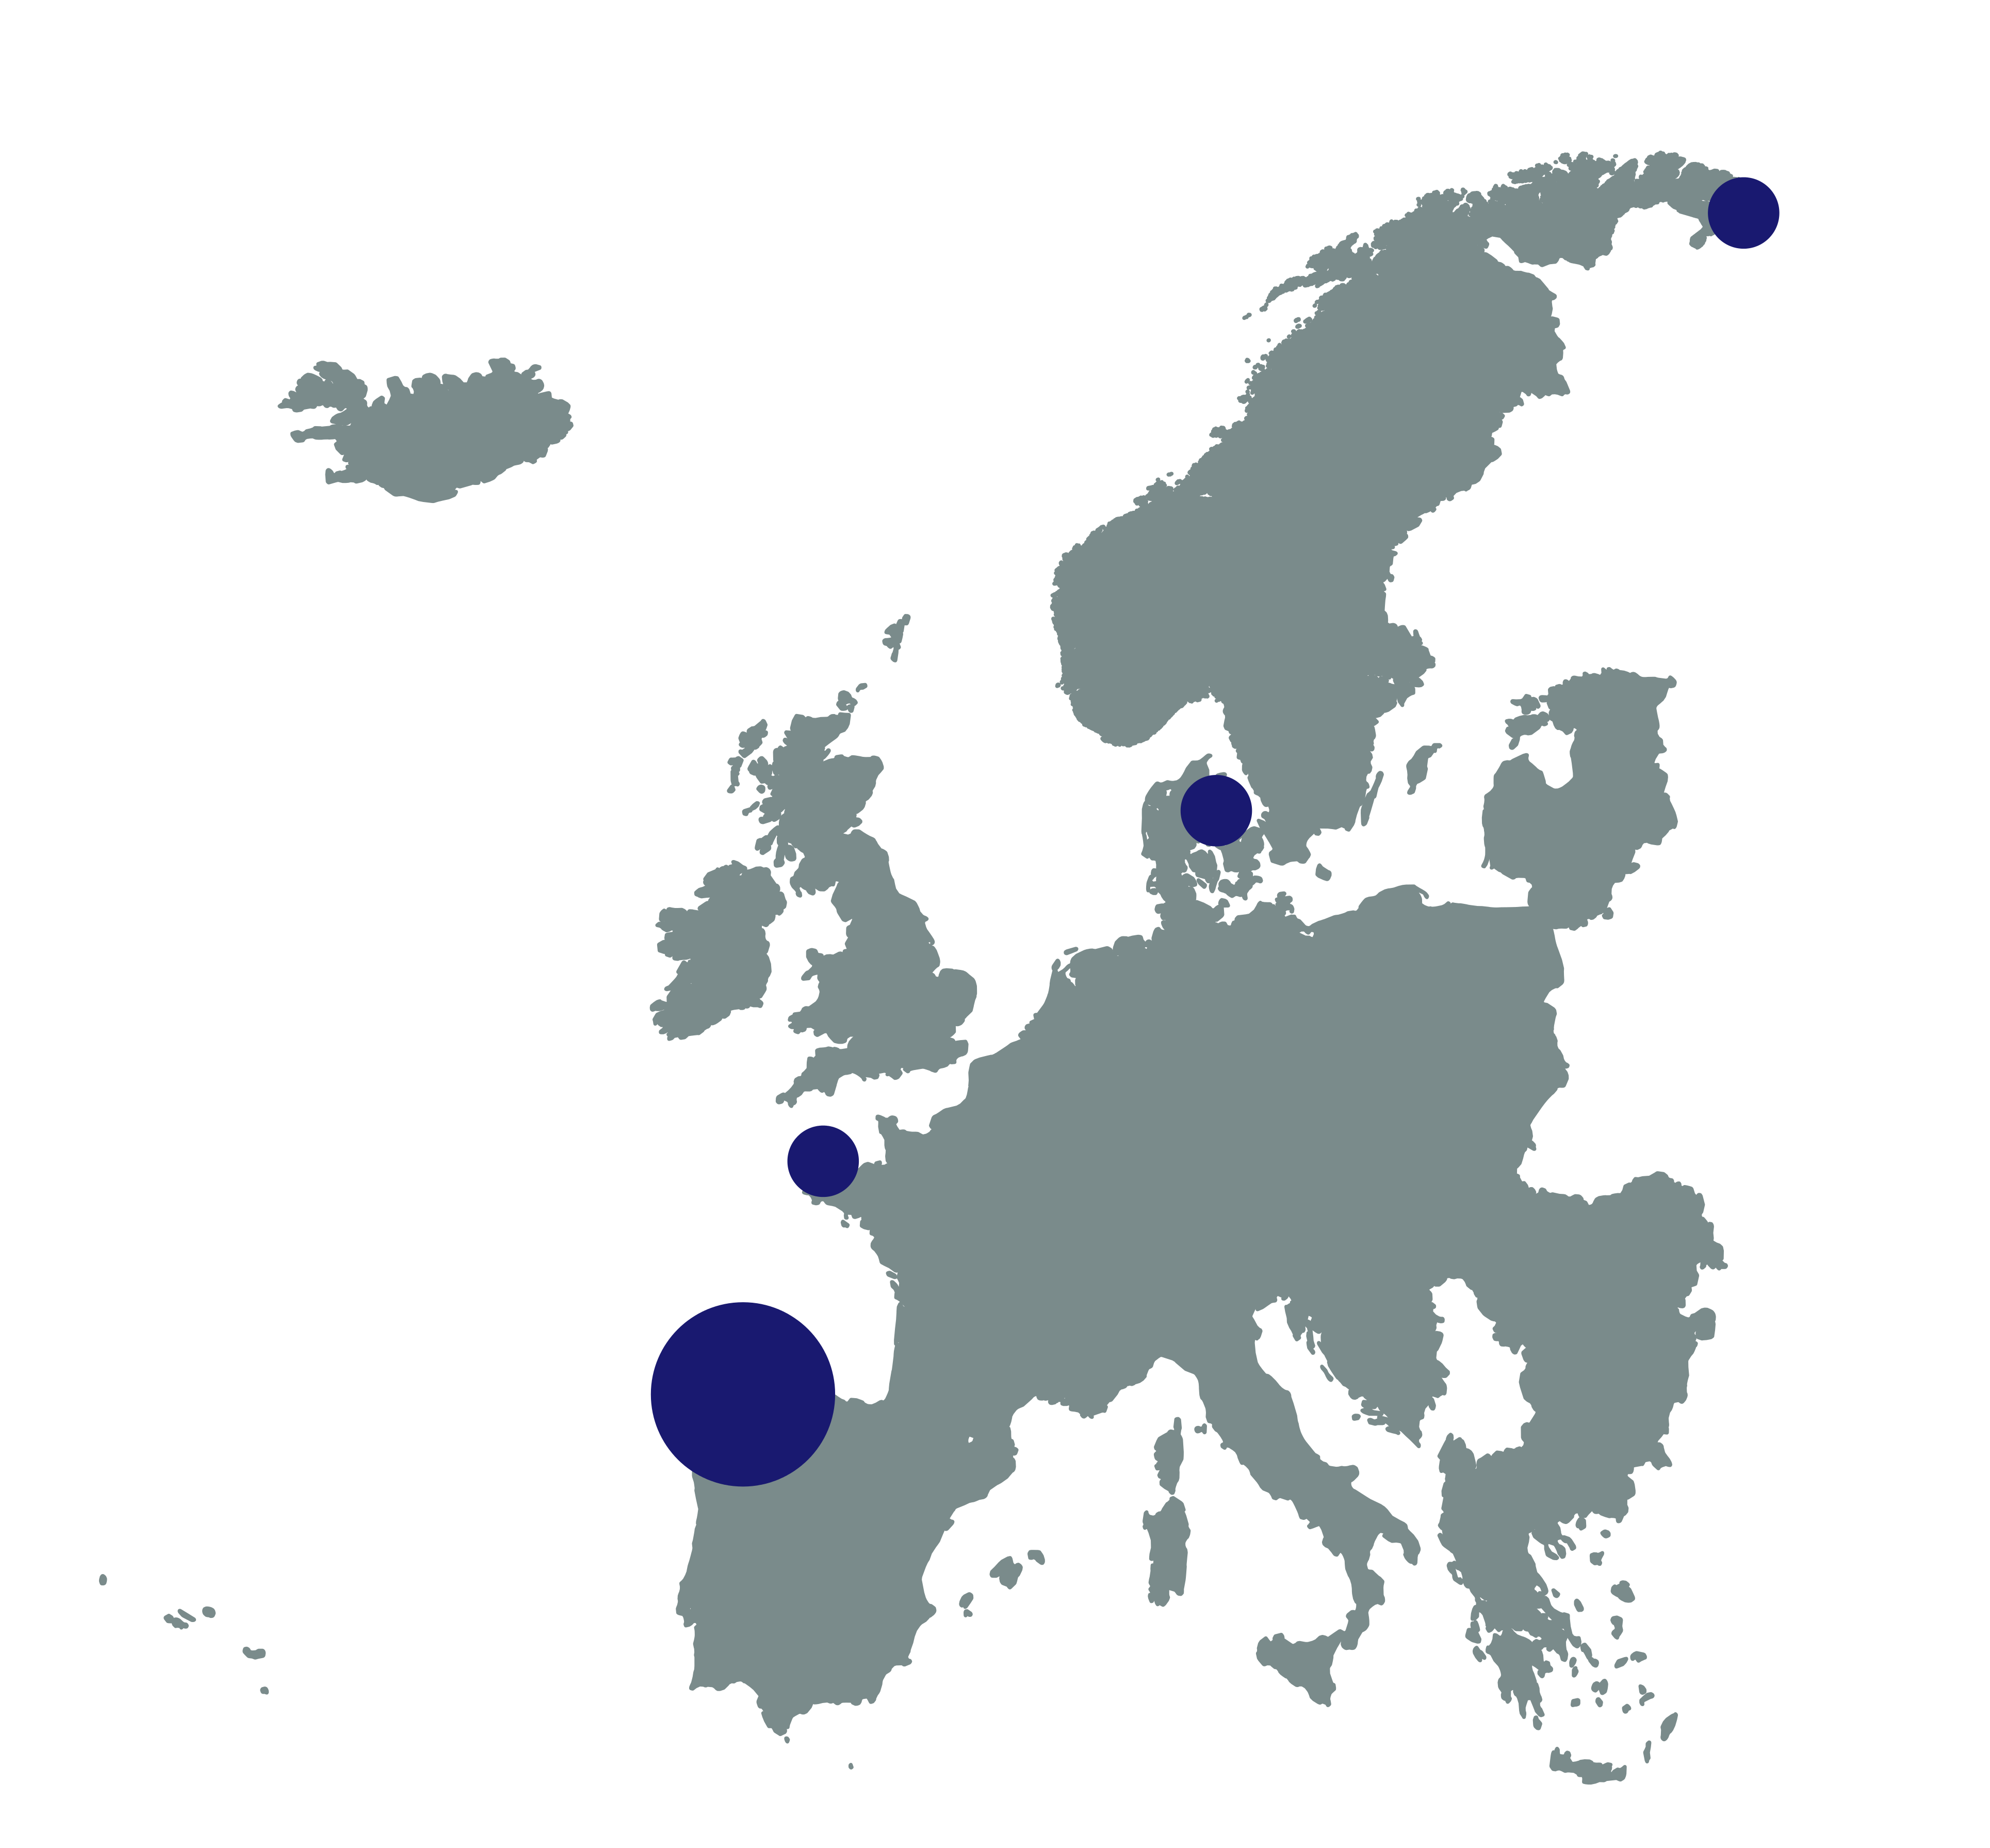
\includegraphics[width=2cm]{Resilience.png}};
\begin{scope}[xshift=2.5cm, yshift=0.5cm]
\draw [color=norway,fill=norway] (4.49,-0.93cm) circle (0.08cm);
\draw [color=denmark,fill=denmark] (3.48,-2.1cm) circle (0.08cm);
\draw [color=france,fill=france] (2.65,-2.8cm) circle (0.08cm);
\draw [color=spain,fill=spain] (2.49,-3.3cm) circle (0.2cm);
\end{scope}
\end{scope}
\draw [color=red!90!black,line width=0.05cm] (4.3cm,-7.5cm) circle (1.2cm);
\node [color=red!90!black] at (3.2cm,-6cm) {\textbf{2}};
\node [color=red!90!black,scale=0.7,text width=3cm,text centered] at (10cm,4.5cm){\textbf{2. Resilience}};
\end{scope}


\end{tikzpicture}

\end{document}